% 2020-04-23 P.Shilane - update template for HotStorage'21
% 2020-09-22 J.Nider - updated template for Systor'21 (acmart.cls v1.73)
% 2022-12-19 Y.Cheng - updated template for HotStorage'23
%
% This file is derived from "sample-sigconf.tex" of the acmart master template
% from 2018/07/16, v1.54
%
% This file should be compiled with
% "acmart.cls", "acmart.dtx", "acmart.ins", "ACM-Reference-Format.bst", v1.54
%
% See "2017 ACM Master Article Template":
% https://www.acm.org/publications/proceedings-template
%

% Do keep the \documentclass "anonymous" parameter until the review process finishes
%\documentclass[sigconf]{acmart}
\documentclass[sigconf,anonymous,10pt]{acmart}


\usepackage{enumitem}
\usepackage{url}
\usepackage{framed}


% Copyright
% Pick the correct copyright notice that matches your rights form
%\setcopyright{none}
\setcopyright{acmcopyright}
%\setcopyright{acmlicensed}
%\setcopyright{rightsretained}
%\setcopyright{usgov}
%\setcopyright{usgovmixed}
%\setcopyright{cagov}
%\setcopyright{cagovmixed}

% DOI
\acmDOI{10.475/1234.5678}

% ISBN
\acmISBN{123-4567-24-567/08/06}

%Conference
\acmConference[HotStorage'23]{15th ACM Workshop on Hot Topics in Storage and File Systems}{July 09, 2023}{in-person conference}
\acmYear{2023}
\copyrightyear{2023}

%\acmArticle{4}
\acmPrice{15.00}

% These commands are optional
%\acmBooktitle{Proccedings of the 13th ACM Workshop on Hot Topics in Storage and File Systems}
%\editor{John Doe}
%\editor{Jane Doe}

\settopmatter{printacmref=false} % Removes citation information below abstract
\renewcommand\footnotetextcopyrightpermission[1]{} % removes footnote with conference information in first column
\pagestyle{plain} % removes running headers

%%%%%%%%%%%%%%%%%%%%%%%%%%%%%%%%%%%%%%%%%%%%%%%%%%%%%%%%%%%%%%%%%%%%%%
%%%%%%%%%%% packages %%%%%%%%%%5
%%%%%%%%%%%%%%%%%%%%%%%%%%%%%%%%%%%%%%%%%%%%%%%%%%%%%%%%%%%%%%%%%%%%%%

\usepackage{tikz}
\usepackage{amsmath, amsfonts}
\usepackage{filecontents}
\usepackage[utf8]{inputenc}
\usepackage{graphicx}
\usepackage{booktabs}
\usepackage{url}
\usepackage{xspace}
\usepackage{microtype}
\usepackage{balance}
% \usepackage{cite}
\usepackage{cleveref}
\usepackage{caption}
\usepackage{subcaption}
\usepackage{flushend}
\usepackage{hyperref}
\usepackage[ruled,vlined]{algorithm2e}
\usepackage[normalem]{ulem}
\usepackage{booktabs}
\usepackage{wrapfig}
\usepackage{flushend}
\usepackage{listings}
\usepackage{float}
\usepackage{enumitem}
\usepackage{comment}
\usepackage{ulem}

\usepackage[T1]{fontenc}
\usepackage[italian]{babel}

%\usepackage{outlines}

\usepackage{blindtext}
\usepackage{etoolbox}


%%%%%%%%%%%%%%%%%%%%%%%%%%%%%%%%%%%%%%%%%%%%%%%%%%%%%%%%%%%%%%%%%%%%%%
%%%%%%%%%%% auxiliarty commands  %%%%%%%%%%5
%%%%%%%%%%%%%%%%%%%%%%%%%%%%%%%%%%%%%%%%%%%%%%%%%%%%%%%%%%%%%%%%%%%%%%


\newcommand{\showcomments}{0}

%-- Provides fixed width font for commands and code snips.
\newcommand{\code}[1]{\texttt{\textbf{#1}}}

%-- Terms...  Use this to introduce a term in the paper.
\newcommand{\term}[1]{\emph{#1}}

%-- Provides stylization for e-mail addresses
%\newcommand{\email}[1]{\emph{(#1)}}

%-- Starts a minor section (puts the title inline w/ the text.
%\newcommand{\minorsection}[1]{\noindent\textbf{#1}:}
\newcommand{\minorsection}[1]{\vspace{\smallskipamount}\noindent\textbf{#1. }}

%-- Jiri caption
\newcommand{\minicaption}[2]{\caption[#1]{\textbf{#1.} #2}}

%-- Units on numbers: 4KB -> \units{4}{KB}
\newcommand{\units}[2]{#1~#2}

%-- Commands...  i.e. WRITE commands.
\newcommand{\command}[1]{{\sc \MakeLowercase{#1}}}

%-- For notes about things that need to be fixed.
\newcommand{\fix}[1]{\marginpar{\LARGE\ensuremath{\bullet}}
    \MakeUppercase{\textbf{[#1]}}}
%-- For adding inline notes to a draft preceded by your initials
%-- E.g., \fixnote{JJW}{What the heck is a foobar?}
\newcommand{\fixnote}[2]{\marginpar{\LARGE\ensuremath{\bullet}}
    {\textbf{[#1:} \textit{#2\,}\textbf{]}}}

%-- Setting margins: \setmargins{left}{right}{top}{bottom}
\newcommand{\setmargins}[4]{
    % Calculations of top & bottom margins
    \setlength\topmargin{#3}
    \addtolength\topmargin{-.5in}  %-- seems like this should be 1, but .5
                                   %-- balances the text top to bottom
    \addtolength\topmargin{-\headheight}
    \addtolength\topmargin{-\headsep}
    \setlength\textheight{\paperheight}
    \addtolength\textheight{-#3}
    \addtolength\textheight{-#4}

    % Calculations of left & right margins
    \setlength\oddsidemargin{#1}
    \addtolength\oddsidemargin{-1in}
    \setlength\evensidemargin{\oddsidemargin}
    \setlength\textwidth{\paperwidth}
    \addtolength\textwidth{-#1}
    \addtolength\textwidth{-#2}
}

%-- For the tabularx environment... Using L, C, R as the column type
%-- will left, center, or right justify the text.

%-- To comment out a swatch of text, use \omitit{blah blah blah}
\long\def\omitit#1{}

%-- Inline title; useful for sub-sub-sections in which you don't want a separate
%-- line for the title.
\newcommand{\inlinesection}[1]{\smallskip\noindent{\textbf{#1.}}}

%-- todo notes

\newenvironment{outlineenv}{\par\color{red}}{\par}
\newcommand{\outline}[1]{\begin{outlineenv}#1\end{outlineenv}}

\newcommand{\todoO}[1]{\textsf{\textbf{\textcolor{Orange}{[[#1]]}}}}
\newcommand{\todoR}[1]{\textsf{\textbf{\textcolor{Red}{[#1]}}}}
\newcommand{\todoU}[1]{\textsf{\textbf{\textcolor{purple}{[[#1]]}}}}
\newcommand{\todoA}[1]{\textsf{\textbf{\textcolor{Yellow}{[[#1]]}}}}
\newcommand{\todoP}[1]{\textsf{\textbf{\textcolor{violet}{[[#1]]}}}}
\newcommand{\todoL}[1]{\textsf{\textbf{\textcolor{Brown}{[[#1]]}}}}
\newcommand{\todoT}[1]{\textsf{\textbf{\textcolor{Green}{[[#1]]}}}}
\newcommand{\outlinetext}[1]{
   \ifthenelse{\equal{\showcomments}{1}}{
      \outline{#1}}{}}
\newcommand{\oyk}[1]{
   \ifthenelse{\equal{\showcomments}{1}}{
      \todoR{oyk: #1}}{}}


\newcommand{\naive}{}% To make sure that \naive isn't already defined    
\def\naive/{na\"{\i}ve}

\newcommand{\para}[1]{\smallskip\noindent{\textbf{#1}}}



% for shepherding process
%\newcommand{\cradded}[1]{\textcolor{blue}{#1}}
% Cross out text
%\newcommand{\crdeleted}[1]{\textcolor{blue}{\sout{#1}}}
% Replace the second argument by the first argument
%\newcommand{\crreplaced}[2]{\textcolor{blue}{\sout{#2}}\textcolor{blue}{#1}}

% for camera ready process
\newcommand{\cradded}[1]{#1}
\newcommand{\crdeleted}[1]{}
\newcommand{\crreplaced}[2]{#1}

% Commands
\newcommand{\myparagraph}[1]{\vspace{\smallskipamount}\noindent\textbf{#1. }}
\newcommand{\eg}{\emph{e.g.}\xspace}
\newcommand{\etc}{etc.\@\xspace}
\newcommand{\cf}{{cf.}\xspace}
\newcommand{\ie}{\emph{i.e.}\xspace}
\newcommand{\etal}{\emph{et al.}\xspace}

\newcommand{\anonAzure}{a large cloud provider\xspace}

\newcommand{\anonFunctions}{a large serverless provider\xspace}

\newcommand{\sys}{Palette\xspace}

% Comment out toggletrue line to generate paper with no comments
\newtoggle{showmarks}
\toggletrue{showmarks}  %%%    <--- comment out this line :)


% side comment
\def\hn{\sffamily\selectfont}
\newcommand{\mpfont}{\hn\scriptsize}
\newcommand{\MPworker}[2]{\unskip{\color{#1}\vrule\vrule}{\marginpar{\raggedright\color{#1}\mpfont #2}}}
\iftoggle{showmarks}{
  \newcommand\mania[1]{\textcolor{magenta}{mania: #1}}
  \newcommand\dsb[1]{\textcolor{green}{DB: #1}}
  \newcommand\rf[1]{\textcolor{cyan}{RF: #1}}
  \newcommand\inigo[1]{\textcolor{red}{IG: #1}}
  \newcommand\gohar[1]{\textcolor{orange}{GOHAR: #1}}
  \newcommand\cheng[1]{\textcolor{blue}{cheng: #1}}
  \newcommand\jiyong[1]{\textcolor{orange}{jy: #1}}
  \newcommand\TODO[1]{\textcolor{blue}{TODO: #1}}

  \newcommand{\CP}[1]{\MPworker{blue}{CT: #1}}
}{
  \newcommand\mania[1]{\unskip}
  \newcommand\daniel[1]{\unskip}
  \newcommand\rf[1]{\unskip}
  \newcommand\inigo[1]{\unskip}
  \newcommand\gohar[1]{\unskip}
  \newcommand\cheng[1]{\unskip}
  \newcommand\jiyong[1]{\unskip}
  \newcommand\TODO[1]{\unskip}

  \newcommand{\CP}[1]{\unskip}
}

\newcommand{\heading}[1]{
  \vspace{1ex}
  \noindent
  \textbf{#1}}

\newcommand{\todo}[1]{{\color{red}#1}}

% names
\newcommand{\sqlite}{SQLite\xspace}
\newcommand{\pmem}{PMem\xspace}
\newcommand{\tuner}{configure tuner\xspace}





\begin{document}

\title{OBFS: a serverless elastic file system}

% Fill in your details. The \documentclass "anonymous" parameter keeps them hidden, remove it after the review process finishes
\author{Leave Empty foFirst1 Last1}
\affiliation{%
  \institution{Institution1}
  \city{City1}
  \state{Country1}
}
\email{email1@mail.com}

\author{First2 Last2}
\affiliation{%
  \institution{Institution2}
  \city{City2}
  \state{Country2}
}
\email{email2@mail.com}

\author{First3 Last3}
\affiliation{%
  \institution{Institution3}
  \city{City3}
  \state{Country3}
}
\email{email3@mail.com}

% The default list of authors is too long for headers.
\renewcommand{\shortauthors}{F. Last1 et al.}

\begin{abstract}
Abstract comes here. 
\end{abstract}

%% Note: Classification and Keywords are only required for the camera-ready version

%
% The code below should be generated by the tool at
% http://dl.acm.org/ccs.cfm
% Please copy and paste the code instead of the example below.
%
%\begin{CCSXML}
%<ccs2012>
%<concept>
%<concept_id>10010520.10010575.10010577</concept_id>
%<concept_desc>Computer systems organization~Reliability</concept_desc>
%<concept_significance>500</concept_significance>
%</concept>
%<concept>
%<concept_id>10010520.10010553.10010562</concept_id>
%<concept_desc>Computer systems organization~Embedded systems</concept_desc>
%<concept_significance>100</concept_significance>
%</concept>
%<concept>
%<concept_id>10010583.10010588.10010592</concept_id>
%<concept_desc>Hardware~External storage</concept_desc>
%<concept_significance>300</concept_significance>
%</concept>
%</ccs2012>
%\end{CCSXML}

%\ccsdesc[500]{Computer systems organization~Reliability}
%\ccsdesc[100]{Computer systems organization~Embedded systems}
%\ccsdesc[300]{Hardware~External storage}
%\ccsdesc[300]{Hardware~Sensor applications and deployments}
%\ccsdesc[300]{Hardware~Wireless integrated network sensors}

%\keywords{ACM proceedings, \LaTeX, text tagging}


% \makeatletter
% \patchcmd{\maketitle}{\@copyrightspace}{}{}{}
% \makeatother
% 
% \usepackage{enumitem}
% \setlist[enumerate,2]{label=\roman*)}
% \setlist[enumerate,3]{label=\alph*)}



\maketitle

\sloppy

\section{Introduction}
\label{sec:intro}

\outline{missing discussions}


\outline{alternatives approaches}
-- EFS and 
-- \mania{Why user should use EFS}


\outline{storage requirement has been shifted from fixed size block storage to elastic }
The emerging computing models such as in-process virtualization such as containers~\cite{docker,kubernetees}, serverless computing such as Azure Functions~\cite{azurefunctions}, and large scale data processing frameworks such as Spark\~cite{spark} is changing the way we traditionally interact with the storage system.
Traditionally, high performance storage preconfigured options such as remove block storage and local SSD has been offered to the application.   
However, these new computing paradigm requires elastic, high performance, durable, and serverless storage options. The current offering of storage options falls short to provide one or some of these requirements. 


\outline{Go through each requirement and talk about why we don't have it}
These emerging computing paradigm requires elastic storage. 
The reason is currently data processing frameworks such as Spark are build using predifined clusters. 
Spark communicates with the storage system in two ways: (1) durable data, (2) ephemeral data. 
For the durable data, the approach is to use a remote distributed storage system such as HDFS or S3 to load store input and output of a job.
For the ephemeral data, the local storage of each compute node is used to store the intermediate data, as well as logs and as a swap space for memory of the workers. 
Typically, for the local storage a preconfigured block device that is local or remote to the computing host is used to store these intermediate temporal data.
However, it is not possible to know apriori how much storage is reuqired to store all of the temporal data. 
When a worker node rans out of space if it is local storage the running task will be failed and it requires manual attention of the cluster administrator to resolve the attached volume. 
One of the reasons that an attached volume could run out of space is the size of the intermediate data which is not known appriori and job configuraiton is done accroding to the first stage of the running job. 
Any further requirement for local storage is bounded by this preconfigured storage. 
Recent studies has shown that the size of this intermediate data can vary drastically and preconfigured storage could falls short to enable running job. 
The solution is to have an elastic storage options that grows and shrinks according to the requirements of the application. 
What we need here is an elastic and high performance storage option. 
Elastic solutions such as Amazon EFS and Skyline provides NFS semantics and requires further modification of the applicaiton to adopt the NFS semantic. 
On the other hand, these alternative elastic solutions provides the consistency across different instances of the file system while this is not a necessary option for applications that only uses file system as a local storage. 
These alternatives imposes extra latency to enable supports the multi client access to the file system.

The second requirement is the requirement to support serverless applications. 
Serverless application or function as a service is a new computing paradigm in which users are responsible to define their code and serverless platform will take care of everything else from resource allocation for application to provision the resources to executing the function. 
One limitation of such system is n these platforms the user has no control over where its job is running thus if the applications require to persist some state locally there is not file system or persistent store that allows the user to do so.
Thus the defacto approach for serverless application is to leverage the external storage such as external key value storage or object storage. 
The challenges is this limitation hinders many serverfull applications to adopt themselves to serverless computing paradigm. Because these applications require extensive modification of their code base to the new object store base API.  
What we need here is a serverless file system that is client side and does not require external storage provisioning such as key value store and support posix api so it does not require extensive modification to the application code base. 



The third requirement is the requirement for elastic file level image store for the containers. 
The recent trend for the containers is that the image that builds the container final image are build by fetching different versions of the storage image overtime. 
There are some solutions that store them as file system but they falls short to provide full posix functionality. 
what they need is a file system that is capable of storage image as file system. 






















\section{Use cases}
\label{sec:usecases}


\subsection{Elastic client-side storage}
\label{sec:usecase:elasticstorage}


\subsection{Container image repository}
\label{sec:usecase:containers}


\subsection{Serverless functions}
\label{sec:usecase:serverless}


\section{Background \& related work}
\label{sec:background}

The closest related work to ObFS is likely ObjectiveFS\footnote{\url{https://objectivefs.com}}, a multi-client file system over S3 which appears to provide NFS-like close-to-open consistency.
Like ObjectiveFS, it uses S3 as a data and metadata store rather than providing 1:1 mapping, achieving performance comparable to or better than NFS, however its structure and algorithms have not been publicly disclosed and are not known to the authors.

Log-structured file systems have a long history, from LFS~\cite{rosenblum_design_1991} and WAFL~\cite{hitz_file_1994} through more recent systems such as F2FS~\cite{lee_f2fs_2015}.
To the authors' knowledge F2FS is the only log-structured file system to date to use write-optimized journaling and recovery-time roll-forward to reduce the cost of metadata updates.
However the use of journaling in F2FS is very limited, as opposed to its pervasive use in ObFS.

The lack of a standard on-media container structure in ObFS is unusual but not unprecedented, and can be compared with BetrFS~\cite{jannen_betrfs_2015} and its use of a schema for data and metadata over an underlying key-value store.
In both cases the lack of directory containers is a result of fundamental architectural decisions, and does not in itself confer any benefits.

Finally, ObFS owes a debt to several decades of research on Flash Translation Layers.
In particular, at the time of development of the first log-structured file systems with garbage collection (e.g. LFS~\cite{rosenblum_design_1991}, Envy~\cite{wu_envy_1994}) there was no prior art for understanding the behavior and costs of garbage collection.
In the time since then great strides have been made in understanding this process, both its risks (i.e. catastrophic performance loss under sustained random write workloads), how to ameliorate them in theory, by segregating data by expected lifetime~\cite{lee_last_2008}, and practical methods for doing so, such as multiple write frontiers~\cite{lee_f2fs_2015} and cleaning hysteresis.

\section{The ObFS File System:\\ Design \& Implementation}
\label{sec:obfs}
ObFS is based on the following principles:

1. Metadata is designed to be used in memory, not from storage.
Files are maps from extents within the file to extents within objects, and directories are maps from names to inode numbers and ancillary information.
Metadata objects are serialized into checkpoints and may then be flushed from memory and demand-loaded later, but the metadata serialization format is not designed to be mutable.

2. Data and metadata is persisted in a stream of objects tagged with sequence numbers as numeric prefixes, allowing efficient internal representation of object names.
Each object encodes a consecutive sequence of file system operations, allowing a consistent prefix to be recovered after failure even if multiple object writes are in progress at the time of failure.

3. Files, directories, and other file system objects (symlinks, special files) are identified by inode number.
These numbers are opaque identifiers and do not identify location, but instead are assigned from an incrementing counter.

4. Each object contains a logical journal of individual file system operations, described below, plus a data region containing the data for write operations in the journal.

\begin{figure}
\begin{framed}
{\footnotesize 
\begin{verbatim}
object "vdisk.0000":
  INODE num=1 mode=S_DIR|0777, size=0, uid/gid, timestamp
  CREATE parent=1 inum=2 name="file.txt"
  INODE num=2  mode=S_REG|0777, uid/gid, size=0, timestamp
  DATA 11 offset=0 dataptr=0 len=15 newsize=15
  --
  this is a test\n
\end{verbatim} }
\end{framed}

  \caption{ A trivial ObFS file system. \rm The root directory is inode 1; it contains a single file, ``file.txt'', with a 15-byte write starting at offset 0 in the object data segment.} 
  %(S\_REG is the POSIX mode flag for a ``regular'' file)}
  \label{figure:journal1}
\end{figure}

\begin{figure}
\begin{framed}
 {\footnotesize
\begin{verbatim}
object "vdisk.0001":
  CREATE parent=1 inum=3 name="dir1"
  INODE num=3 mode=S_DIR|0777, uid/gid, size=0, timestamp
  DATA num=2 offset=15 dataptr=0 len=15 newsize=40
  --
  this is another test\n
\end{verbatim} }
\end{framed}
  \caption{Second data object. \rm Creates subdirectory \texttt{/dir1} and adds 15 bytes to \texttt{/file.txt}.}
  \label{figure:journal2}
\end{figure}


\begin{figure}
\centering
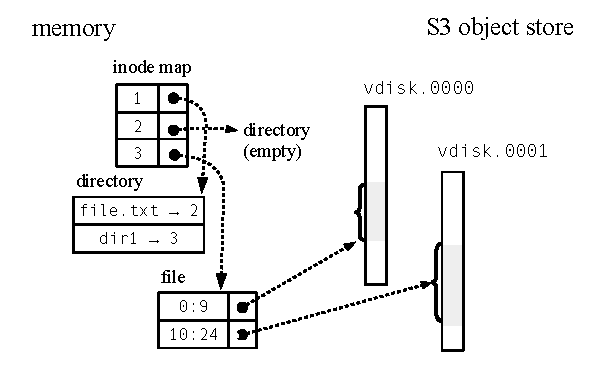
\includegraphics[width=0.95\columnwidth]{figs/obfs.pdf}
\caption{Relationship of in-memory structures and S3 objects for file system shown in Figures \ref{figure:journal1} and \ref{figure:journal2}.}
\label{figure:picture}
\end{figure}

\subsection{Logical Journal Format}

A trivial example of an ObFS file system may be seen in Figure~\ref{figure:journal1}.
It contains a journal of the following operations:
\begin{itemize}[nosep]
\item Modify root directory properties (inode 1) to set permissions, UID/GID, and timestamp
\item Create an entry for a new file, \texttt{/file.txt} in the root directory
\item Set inode properties for the file
\item Write 15 bytes to the file
\end{itemize}

At mount time the log will be replayed; when complete the root directory will have a single entry [\texttt{"file.txt"} $\rightarrow$ 2], and the file identified as inode 2 will have a single extent in its map, with offsets $[0\ldots 14]$ mapped to offset 0 in the data section of object 0.
In Figure~\ref{figure:journal2} we see the second object in the stream, journaling the creation of an empty directory (\texttt{/dir1}) and the write of 15 more bytes to \texttt{/file.txt}; again these will be reflected in in-memory data structures after journal recovery during the mount process.

\begin{table}
  \begin{tabular}{l|l}
    Operation & \rule{4em}{0pt} arguments \\
    \hline
    INODE & inum, mode, uid/gid, rdev, mtime \\
    CREATE & parent inum, inum, name \\
    RENAME & inum, parent inum1, inum2, name1, name2 \\
    TRUNC & inum, new size\\
    DELETE & parent inum, inum, name \\
    SYMLINK & inum, target\\
    DATA & inum, file offset/len, obj offset, new file size\\
    \hline
  \end{tabular} \vspace{0.5\baselineskip}
  \caption{ObFS journal entry types}
  \label{table:journal}
\end{table}

The full list of seven journal entry types may be seen in Table~\ref{table:journal}.
We believe that they are sufficient for basic POSIX file system functionality, although our implementation has taken some liberties with timestamps (we assume \texttt{noatime} mounts) and we have not yet implemented reference counting for hard links in either the in-memory or serialized metadata formats.

Figures~\ref{figure:journal1} and \ref{figure:journal2} show back-end storage objects which are ridiculously small, for illustrative purposes.
In practice objects would be written when either (a) a default size has been reached (e.g. 8-16\,MiB), (b) an idle timeout has passed (e.g. 1s), or (c) a synchronizing operation (\texttt{fsync}, etc.) is performed.
The file system may be operated in an unsafe mode by either ignoring synchronizing operations entirely, in which case failure may cause data and operation loss but will not result in an inconsistent file system, or by logging to local high-speed storage, in which case synchronized data may be lost in the case of catastrophic failures.

\subsection{In-memory metadata}
Although in-memory data structures for a file system may be considered implementation details rather than architecture, their functionality is central to the architecture of ObFS.
Our description of these structures is provided in order to explain this functionality in a straightforward fashion, rather than to constrain implementation\footnote{For instance, in a proper in-kernel VFS implementation the structures described would no doubt be ``absorbed'' into existing kernel data structures.}.

ObFS supports the standard UNIX/POSIX file system objects: files, directories, symbolic links, and various classes of special files (e.g. character devices) with no file system functionality.
All objects (in the OO sense) have basic metadata such as uid/gid and timestamps; with the addition of a device number this is sufficient for the special file types.
This object is extended with the following information for the remaining types:
\begin{itemize}[nosep]
\item \textbf{Symbolic link:} a single string, the link target.
\item \textbf{Directory:} a map from strings (i.e. names) to integer inode numbers.
\item \textbf{File:} a byte-granularity interval map from offset ranges within the file to (object, offset) pairs indicating the location of the data in an S3 object\footnote{We explicitly call these ``S3 objects'' here to differentiate from in-memory objects, however other S3-like services providing named objects may of course be used.} from storage objects; however , with S3 objects identified by their integer sequence number.
\end{itemize}

Finally an inode table is used to map inode numbers to objects; path traversal thus iterates between accesses to this table and to individual directories.

\subsection{Checkpoints}

If ObFS were to do nothing but log operations to storage then mounting a file system would soon become unwieldy, requiring the playback of all operations performed on the file system to date.
To avoid this we periodically checkpoint metadata to storage so that the file system may be mounted by locating the most recent checkpoint, loading that into memory, and then rolling the journal forward from that point.
Note that a clean unmount will perform a checkpoint after all writes are complete, eliminating any recover overhead at mount time.

As the file system grows, the memory requirements for in-memory metadata may grow excessive.
This may be addressed by demand-loading metadata from the most recent checkpoint, and evicting unmodified metadata objects from memory when necessary.
This requires a mechanism to map an inode number to its location in the checkpoint: the two obvious possibilities are (a) a mapping table in the checkpoint, or (b) appending the information to directory entries.
Our current design stores an inode number to location map in the checkpoint, in part because this mapping is needed during garbage collection, when the identity of the parent directory may not be known.
We expect to revisit this decision as we gain experience with larger file systems, as performance may suffer if this table grows too large to be held in memory.

With further growth of a file system the overhead of writing checkpoints will increase.
If a fixed checkpoint interval is maintained, then metadata write overhead will go up as the ratio of modified to total metadata shrinks.
However, if the checkpoint interval is allowed to expand proportionally to reduce this overhead, mount time will suffer.

This may be addressed by keeping multiple partial snapshots.
Rather than implementing a complex garbage collection mechanism we use a simple FIFO method, keeping the last N checkpoints and copying any un-replicated data from the oldest checkpoint when we make a new one.
The need to keep separate inode maps for each snapshot limits the number of snapshots which may be maintained in practice, and alternate methods may be needed to support volumes of more than a few tens of millions of files.

\subsection{Garbage Collection}

ObFS has been tested with a simple Greedy cleaning algorithm, selecting the least-utilized objects, reading and re-writing any remaining live data before object deletion.
This is known to be optimal for uniform memoryless workloads~\cite{yang_optimality_2015}, but to perform poorly when workloads are skewed or correlated~\cite{desnoyers_analytic_2014}. 
We therefore include several well-known techniques which greatly improve its performance on realistic workloads:

\textbf{Dual write frontiers:}~\cite{lin_dual_2012} In realistic workloads, data which has survived long enough to be copied during garbage collection has a longer expected time-to-live than new writes.
  ObFS garbage collection output is written into separate objects, implicitly performing hot/cold data segregation.

\textbf{Write coalescing:} The hottest data items will be overwritten before an object is written to storage.
  By merging data and metadata in an object before it is written out, this space may be reclaimed without any copying, or even writing it in the first place\footnote{This is not yet implemented in our prototype.}.

\textbf{Hysteresis-based batching:} Optimal cleaning of skewed workloads requires allowing blocks containing hot data to ``age'' to lower utilizations than those containing cold data~\cite{desnoyers_analytic_2014}.
  To do this optimally requires extensive bookkeeping; however in practice the simple hysteresis mechanism we use achieves most of its benefits, deferring cleaning until a low-water mark is reached, then cleaning until a high-water mark is reached.

To identify live data we read the DATA records from the object header, and for each check that the current extent map still refers to the same location.
If the relevant inode is in memory it may be looked up directly; if not, the inode location map is used to demand-load it.
Although not implemented in our current prototype, we plan to segregate metadata loaded for garbage collection and free it at the end of the cycle.

Finally we note that ObFS objects contain metadata such as directory and inode information (e.g. CREATE and INODE records) as well as data.
Garbage collection must therefore either (a) only consider objects for deletion which are older than the most recent full checkpoint, or (b) create a new checkpoint before deletion.
Our current prototype chooses option (b), checkpointing metadata before beginning a garbage collection cycle.

\subsection{Additional features}
We are extending ObFS to support snapshots, clones of a base file system image, and "native overlay"---a form of clone based on multiple parent file systems.
We describe these briefly due to space limitations.

\noindent \textbf{Cloning:} The object stream for a cloned volume looks almost exactly like that for a simple ObFS file system, with objects older than a certain sequence number belonging to the base image, and later objects belonging to the clone, using a different prefix for object names.

\noindent \textbf{Snapshots:} A snapshot is just a specific object in the stream and its predecessors.
Garbage collection continues in the presence of snapshots; however objects containing data referenced by snapshots are not deleted until those snapshots have been removed.

\noindent \textbf{Overlay:} This is performed via an ordered merge of the metadata from several underlying file systems\footnote{This involves translating inode numbers and object sequence numbers; lack of space prohibits a full explanation.}, which may then be written as the initial checkpoint of the merged volume.
Although this is a heavier-weight process than union mount, the resulting file system will operate at native speed.

%\cite{10.1109/SMARTCOMP.2014.7043841}

\section{Evaluation}
\label{sec:evaluation}

Our ObFS prototype is a FUSE file system implemented in roughly 2000 lines of C++.
It performs garbage collection and checkpointing, but does not yet implement snapshots, clone, overlays, or partial checkpoints.
We have verified its functionality against a local S3 object store\footnote{Based on Ceph Rados Gateway (RGW).}, but do not yet have performance results.

\section{Discussion}
\label{sec:discussion}
\section{Conclusion}
\label{sec:conclusion}





%\section*{Acknowledgments}
%Acknowledgments are for the camera-ready version only. Please do not include them in your submission.

\bibliographystyle{ACM-Reference-Format}
\bibliography{ref}
\end{document}
